\documentclass{article}

% content/resources/templates/preamble.tex
\usepackage[margin=0.6in]{geometry}
\author{Milav Dabgar}
\usepackage{amsmath,amssymb,amsthm}
\usepackage{booktabs}
\usepackage{multirow}
\usepackage{xcolor}
\usepackage{tcolorbox}
\tcbuselibrary{breakable,skins}
\usepackage[colorlinks=true,linkcolor=blue]{hyperref}
\usepackage{titlesec}
\usepackage{enumitem}
\usepackage{tikz}
\usepackage{pgfplots}
\usepackage{circuitikz}
\usepackage[version=4]{mhchem}
\usepackage{longtable}
\usepackage{array}
\usepackage{float}
\usepackage{caption}
\usepackage{listings}

\lstset{
  basicstyle=\small\ttfamily,
  breaklines=true,
  breakatwhitespace=false,
  postbreak=\mbox{\textcolor{red}{$\hookrightarrow$}\space},
  float=false,
  numbers=left,
  numberstyle=\tiny\color{gray},
  numbersep=10pt,
  xleftmargin=2em,
  keywordstyle=\color{blue},
  commentstyle=\color{green!60!black},
  stringstyle=\color{purple},
  backgroundcolor=\color{gray!5},
  showstringspaces=false,
  tabsize=2,
  captionpos=b,
  keepspaces=true,
  columns=flexible
}

\pgfplotsset{compat=1.18}
\usetikzlibrary{shapes,arrows,positioning,calc,patterns,decorations.pathmorphing,decorations.markings,arrows.meta}

% Color scheme
\definecolor{headcolor}{RGB}{0,102,204}
\definecolor{keycolor}{RGB}{220,20,60}
\definecolor{solutioncolor}{RGB}{34,139,34}
\definecolor{mnemoniccolor}{RGB}{148,0,211}
\definecolor{codecolor}{RGB}{0,0,100}

% Spacing
\setlength{\parskip}{3pt}
\setlist[itemize]{nosep}
\setlist[enumerate]{nosep}

% Title formatting
\titleformat{\section}{\Large\bfseries\color{headcolor}}{\thesection}{1em}{}
\titleformat{\subsection}{\large\bfseries\color{headcolor}}{\thesubsection}{1em}{}

% Pandoc tightlist compatibility
\providecommand{\tightlist}{%
  \setlength{\itemsep}{0pt}\setlength{\parskip}{0pt}}

% Pandoc longtable compatibility
\newcounter{none}
\def\thenone{}


% content/resources/templates/english-boxes.tex

% Custom environments
\newtcolorbox{solutionbox}{
 breakable,
 enhanced,
 colback=solutioncolor!5!white,
 colframe=solutioncolor!75!black,
 fonttitle=\bfseries,
 title=Solution
}

\newtcolorbox{solutionboxnobreak}{
 colback=solutioncolor!5!white,
 colframe=solutioncolor!75!black,
 fonttitle=\bfseries,
 title=Solution
}

\newtcolorbox{keyformula}{
 breakable,
 enhanced,
 colback=keycolor!5!white,
 colframe=keycolor!75!black,
 fonttitle=\bfseries,
 title=Key Formula
}

\newtcolorbox{mnemonicboxenv}{
 breakable,
 enhanced,
 colback=mnemoniccolor!5!white,
 colframe=mnemoniccolor!75!black,
 fonttitle=\bfseries,
 title=Mnemonic
}

\newcommand{\mnemonicbox}[1]{%
  \begin{mnemonicboxenv}
    #1
  \end{mnemonicboxenv}
}


% Custom commands for GTU solutions
% This file defines semantic commands for consistent formatting

% Question command with automatic formatting
\newcommand{\question}[2]{%
  \section*{Question #1}%
  \textbf{#2}%
}

% OR question variant
\newcommand{\questionor}[2]{%
  \section*{Question #1 OR}%
  \textbf{#2}%
}

% Proper table environment with caption
\newenvironment{answertable}[1]{%
  \begin{table}[htbp]
  \centering
  \caption{#1}
}{%
  \end{table}
}

% Proper figure environment for diagrams
\newenvironment{answerdiagram}[1]{%
  \begin{figure}[htbp]
  \centering
  \caption{#1}
}{%
  \end{figure}
}

% Semantic markup for key terms
\newcommand{\keyword}[1]{\textbf{#1}}
\newcommand{\code}[1]{\texttt{#1}}
\newcommand{\classname}[1]{\texttt{#1}}
\newcommand{\methodname}[1]{\texttt{#1}}

% Proper quotation marks
\newcommand{\mnemonic}[1]{``#1''}


\title{Principles of Electronic Communication (4331104) - Summer 2025 Solution}
\date{May 17, 2025}

\begin{document}
\maketitle

\questionmarks{1}{a}{3}
\textbf{Compare Analog Signal and Digital Signal.}

\begin{solutionbox}
    \textbf{Answer}:

    \begin{center}
    \begin{tabulary}{\linewidth}{L L L}
        \toprule
        \textbf{Parameter} & \textbf{Analog Signal} & \textbf{Digital Signal} \\
        \midrule
        \textbf{Nature} & Continuous waveform & Discrete values (0 and 1) \\
        \textbf{Amplitude} & Infinite variations & Fixed discrete levels \\
        \textbf{Noise Effect} & More susceptible & Less susceptible \\
        \textbf{Bandwidth} & Requires less bandwidth & Requires more bandwidth \\
        \textbf{Security} & Less secure & More secure \\
        \bottomrule
    \end{tabulary}
    \end{center}

    \begin{itemize}
        \item \textbf{Signal Type}: Analog signals are continuous, Digital signals are discrete.
        \item \textbf{Noise Resistance}: Digital signals have better noise immunity.
    \end{itemize}

    \begin{mnemonicbox}
    "ABCD - Analog Bad for noise, Continuous; Digital Discrete, Clean signals"
    \end{mnemonicbox}
\end{solutionbox}

\questionmarks{1}{b}{4}
\textbf{Compare PAM, PWM and PPM.}

\begin{solutionbox}
    \textbf{Answer}:

    \begin{center}
    \begin{tabulary}{\linewidth}{L L L L}
        \toprule
        \textbf{Parameter} & \textbf{PAM} & \textbf{PWM} & \textbf{PPM} \\
        \midrule
        \textbf{Full Form} & Pulse Amplitude Modulation & Pulse Width Modulation & Pulse Position Modulation \\
        \textbf{Modulated Parameter} & Amplitude & Width/Duration & Position/Time \\
        \textbf{Noise Immunity} & Poor & Good & Excellent \\
        \textbf{Bandwidth} & Minimum & Medium & Maximum \\
        \textbf{Power Consumption} & High & Medium & Low \\
        \bottomrule
    \end{tabulary}
    \end{center}

    \textbf{Diagram:}

    \begin{center}
    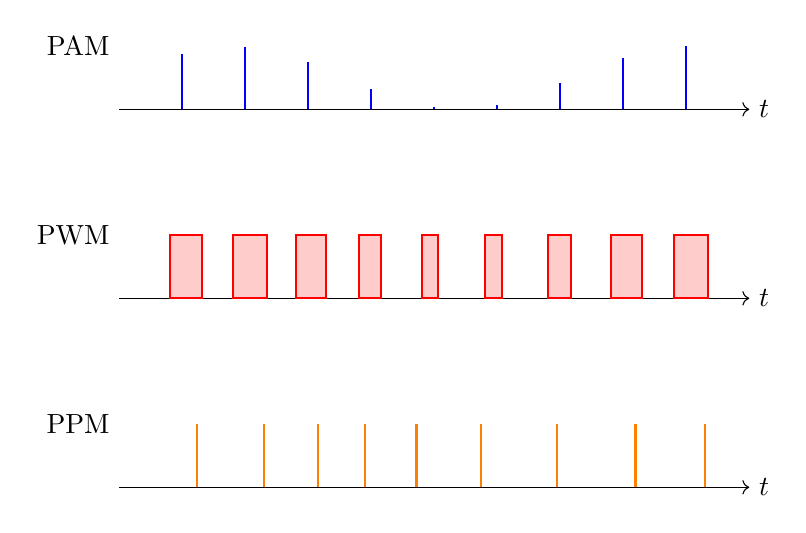
\begin{tikzpicture}[scale=0.8]
        % PAM
        \node [left] at (0, 7) {PAM};
        \draw [->] (0, 6) -- (10, 6) node[right] {$t$};
        \foreach \x in {1,2,3,4,5,6,7,8,9} {
             \pgfmathsetmacro{\yval}{6 + 0.5 + 0.5*sin(\x*50)}
             \draw [thick, blue] (\x, 6) -- (\x, \yval);
        }
        
        % PWM
        \node [left] at (0, 4) {PWM};
        \draw [->] (0, 3) -- (10, 3) node[right] {$t$};
        \foreach \x in {1,2,3,4,5,6,7,8,9} {
            \pgfmathsetmacro{\width}{0.2 + 0.15*sin(\x*50)}
            \draw [thick, red, fill=red!20] (\x-0.2, 3) rectangle (\x+\width, 4);
        }
            
        % PPM
        \node [left] at (0, 1) {PPM};
        \draw [->] (0, 0) -- (10, 0) node[right] {$t$};
        \foreach \x in {1,2,3,4,5,6,7,8,9} {
            \pgfmathsetmacro{\shift}{0.3*sin(\x*50)}
            \draw [thick, orange] (\x+\shift, 0) -- (\x+\shift, 1);
        }
    \end{tikzpicture}
    \end{center}

    \begin{itemize}
        \item \textbf{Modulation Parameter}: Each type modulates different pulse characteristics.
        \item \textbf{Applications}: PWM used in motor control, PPM in radio control systems.
    \end{itemize}

    \begin{mnemonicbox}
    "PAM-Amplitude, PWM-Width, PPM-Position - AWP"
    \end{mnemonicbox}
\end{solutionbox}

\questionmarks{1}{c}{7}
\textbf{Indicate the need of Modulation in detail. Calculate the height of antenna if the frequency of Carrier signal is 1 MHz.}

\begin{solutionbox}
    \textbf{Answer}:

    \textbf{Need for Modulation:}

    \begin{center}
    \begin{tabulary}{\linewidth}{L L}
        \toprule
        \textbf{Reason} & \textbf{Explanation} \\
        \midrule
        \textbf{Antenna Size Reduction} & Makes practical antenna sizes possible \\
        \textbf{Frequency Translation} & Shifts signal to suitable frequency range \\
        \textbf{Multiplexing} & Allows multiple signals on same medium \\
        \textbf{Noise Reduction} & Improves signal-to-noise ratio \\
        \textbf{Power Efficiency} & Better power utilization \\
        \bottomrule
    \end{tabulary}
    \end{center}

    \textbf{Antenna Height Calculation:} \\
    For efficient radiation, antenna height = $\lambda/4$

    \[ \lambda = \frac{c}{f} = \frac{3 \times 10^8}{1 \times 10^6} = 300 \text{ meters} \]

    \[ \textbf{Antenna height} = \frac{\lambda}{4} = \frac{300}{4} = \textbf{75 meters} \]

    \begin{itemize}
        \item \textbf{Practical Antenna}: Without modulation, antenna would be impractically large.
        \item \textbf{Frequency Shifting}: Allows better propagation characteristics.
    \end{itemize}

    \begin{mnemonicbox}
    "AFMNP - Antenna, Frequency, Multiplexing, Noise, Power"
    \end{mnemonicbox}
\end{solutionbox}

\orquestions

\questionmarks{1}{c}{7}
\textbf{Write frequency bands with applications domains of EM Wave spectrum. Calculate Wavelength range of ELF band.}

\begin{solutionbox}
    \textbf{Answer}:

    \begin{center}
    \begin{tabulary}{\linewidth}{L L L L}
        \toprule
        \textbf{Band} & \textbf{Frequency Range} & \textbf{Wavelength} & \textbf{Applications} \\
        \midrule
        \textbf{ELF} & 30-300 Hz & $10^6-10^7$ m & Submarine communication \\
        \textbf{VLF} & 3-30 kHz & $10^4-10^5$ m & Navigation, time signals \\
        \textbf{LF} & 30-300 kHz & $10^3-10^4$ m & AM broadcasting \\
        \textbf{MF} & 300 kHz-3 MHz & 100-1000 m & AM radio \\
        \textbf{HF} & 3-30 MHz & 10-100 m & Short wave radio \\
        \bottomrule
    \end{tabulary}
    \end{center}

    \textbf{ELF Wavelength Calculation:}

    \begin{itemize}
        \item Lower frequency: $f_1 = 30 \text{ Hz}, \lambda_1 = c/f_1 = (3 \times 10^8)/30 = \textbf{10}^7 \textbf{ meters}$
        \item Upper frequency: $f_2 = 300 \text{ Hz}, \lambda_2 = c/f_2 = (3 \times 10^8)/300 = \textbf{10}^6 \textbf{ meters}$
    \end{itemize}

    \textbf{ELF Wavelength range: $10^6$ to $10^7$ meters}

    \begin{itemize}
        \item \textbf{Application Domain}: Each band suited for specific applications.
        \item \textbf{Propagation}: Lower frequencies have better ground wave propagation.
    \end{itemize}

    \begin{mnemonicbox}
    "Every Valuable Learning Makes Happiness - ELF to HF bands"
    \end{mnemonicbox}
\end{solutionbox}

\questionmarks{2}{a}{3}
\textbf{Compare AM and FM.}

\begin{solutionbox}
    \textbf{Answer}:

    \begin{center}
    \begin{tabulary}{\linewidth}{L L L}
        \toprule
        \textbf{Parameter} & \textbf{AM} & \textbf{FM} \\
        \midrule
        \textbf{Modulated Parameter} & Amplitude & Frequency \\
        \textbf{Bandwidth} & 2$f_m$ & $2(\Delta f + f_m)$ \\
        \textbf{Noise Immunity} & Poor & Good \\
        \textbf{Power Efficiency} & Low (33.33\%) & High \\
        \textbf{Circuit Complexity} & Simple & Complex \\
        \bottomrule
    \end{tabulary}
    \end{center}

    \begin{itemize}
        \item \textbf{Bandwidth}: FM requires much wider bandwidth than AM.
        \item \textbf{Quality}: FM provides better audio quality.
    \end{itemize}

    \begin{mnemonicbox}
    "AM-Amplitude simple, FM-Frequency complex but better quality"
    \end{mnemonicbox}
\end{solutionbox}

\questionmarks{2}{b}{4}
\textbf{Draw waveform of Amplitude Modulated wave.}

\begin{solutionbox}
    \textbf{Answer}:

    \textbf{Diagram:}

    \begin{center}
    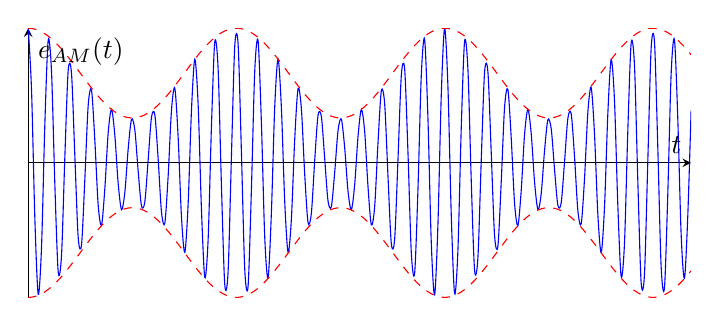
\begin{tikzpicture}
        \begin{axis}[
            width=10cm, height=5cm,
            axis lines=middle,
            xtick=\empty, ytick=\empty,
            xlabel=$t$, ylabel=$e_{AM}(t)$,
            domain=0:20, samples=200
        ]
            \addplot[blue, smooth] {(1 + 0.5*cos(deg(x))) * cos(deg(10*x))};
            \addplot[red, dashed, smooth] {1 + 0.5*cos(deg(x))};
            \addplot[red, dashed, smooth] {-(1 + 0.5*cos(deg(x)))};
        \end{axis}
    \end{tikzpicture}
    \end{center}

    \textbf{Characteristics:}

    \begin{itemize}
        \item \textbf{Envelope}: The envelope follows the modulating signal.
        \item \textbf{Carrier Frequency}: Remains constant throughout.
        \item \textbf{Amplitude Variation}: Amplitude varies with modulating signal.
    \end{itemize}

    \begin{mnemonicbox}
    "Envelope Follows Message - EFM"
    \end{mnemonicbox}
\end{solutionbox}

\questionmarks{2}{c}{7}
\textbf{Define Amplitude Modulation and Derive mathematical expression for Double Sideband Full Carrier (DSBFC) Amplitude Modulation (AM) signal.}

\begin{solutionbox}
    \textbf{Answer}:

    \textbf{Definition:} Amplitude Modulation is the process where amplitude of carrier signal varies according to instantaneous amplitude of modulating signal.

    \textbf{Mathematical Derivation:}

    Let carrier signal: $e_c(t) = E_c \cos(\omega_c t)$ \\
    Let modulating signal: $e_m(t) = E_m \cos(\omega_m t)$

    \textbf{AM Signal Expression:}
    \[ e_{AM}(t) = [E_c + E_m \cos(\omega_m t)] \cos(\omega_c t) \]
    \[ e_{AM}(t) = E_c \cos(\omega_c t) + E_m \cos(\omega_m t) \cos(\omega_c t) \]

    Using trigonometric identity:
    \[ \cos A \cos B = \frac{1}{2}[\cos(A+B) + \cos(A-B)] \]

    \textbf{Final AM Expression:}
    \[ e_{AM}(t) = E_c \cos(\omega_c t) + \frac{E_m}{2} \cos(\omega_c + \omega_m)t + \frac{E_m}{2} \cos(\omega_c - \omega_m)t \]

    \textbf{Components:}

    \begin{itemize}
        \item \textbf{Carrier Component}: $E_c \cos(\omega_c t)$
        \item \textbf{Upper Sideband}: $\frac{E_m}{2} \cos(\omega_c + \omega_m)t$
        \item \textbf{Lower Sideband}: $\frac{E_m}{2} \cos(\omega_c - \omega_m)t$
    \end{itemize}

    \begin{mnemonicbox}
    "Carrier Plus Upper Lower Sidebands - CPULS"
    \end{mnemonicbox}
\end{solutionbox}

\orquestions

\questionmarks{2}{a}{3}
\textbf{Compare Pre-emphasis and De-emphasis.}

\begin{solutionbox}
    \textbf{Answer}:

    \begin{center}
    \begin{tabulary}{\linewidth}{L L L}
        \toprule
        \textbf{Parameter} & \textbf{Pre-emphasis} & \textbf{De-emphasis} \\
        \midrule
        \textbf{Location} & At transmitter & At receiver \\
        \textbf{Function} & Boosts high frequencies & Attenuates high frequencies \\
        \textbf{Frequency Response} & High pass characteristic & Low pass characteristic \\
        \textbf{Purpose} & Improve S/N ratio & Restore original signal \\
        \textbf{Time Constant} & 75 $\mu$s (FM broadcasting) & 75 $\mu$s (FM broadcasting) \\
        \bottomrule
    \end{tabulary}
    \end{center}

    \begin{itemize}
        \item \textbf{Noise Reduction}: Combined effect reduces noise in received signal.
        \item \textbf{Frequency Response}: Complementary characteristics.
    \end{itemize}

    \begin{mnemonicbox}
    "Pre-Boost, De-Cut - Noise Reduction Circuit"
    \end{mnemonicbox}
\end{solutionbox}

\questionmarks{2}{b}{4}
\textbf{Draw waveform of Frequency Modulated wave.}

\begin{solutionbox}
    \textbf{Answer}:

    \textbf{Diagram:}

    \begin{center}
    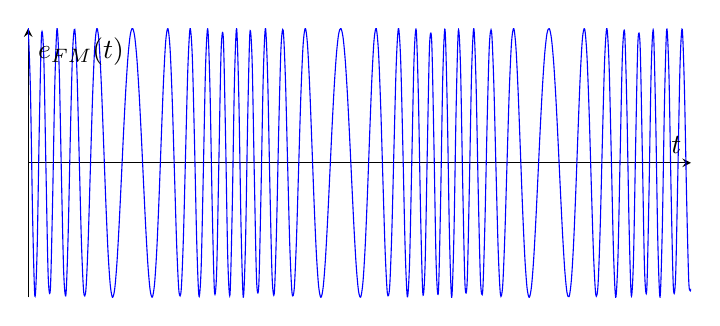
\begin{tikzpicture}
        \begin{axis}[
            width=10cm, height=5cm,
            axis lines=middle,
            xtick=\empty, ytick=\empty,
            xlabel=$t$, ylabel=$e_{FM}(t)$,
            domain=0:20, samples=300
        ]
            % FM wave: cos(wc t + mf sin(wm t))
            \addplot[blue, smooth] {cos(deg(10*x + 5*sin(deg(x))))};
        \end{axis}
    \end{tikzpicture}
    \end{center}

    \textbf{Characteristics:}

    \begin{itemize}
        \item \textbf{Constant Amplitude}: Amplitude remains constant.
        \item \textbf{Frequency Variation}: Frequency varies with modulating signal.
        \item \textbf{Phase Continuity}: Phase remains continuous.
    \end{itemize}

    \begin{mnemonicbox}
    "Constant Amplitude, Variable Frequency - CAVF"
    \end{mnemonicbox}
\end{solutionbox}

\questionmarks{2}{c}{7}
\textbf{Define Frequency Modulation and Derive mathematical expression for FM wave.}

\begin{solutionbox}
    \textbf{Answer}:

    \textbf{Definition:} Frequency Modulation is the process where frequency of carrier signal varies according to instantaneous amplitude of modulating signal.

    \textbf{Mathematical Derivation:}

    Let modulating signal: $e_m(t) = E_m \cos(\omega_m t)$ \\
    Instantaneous frequency: $f_i = f_c + k_f E_m \cos(\omega_m t)$

    Where $k_f$ = frequency sensitivity

    \textbf{Instantaneous angular frequency:}
    \[ \omega_i = 2\pi[f_c + k_f E_m \cos(\omega_m t)] \]
    \[ \omega_i = \omega_c + 2\pi k_f E_m \cos(\omega_m t) \]

    \textbf{Phase calculation:}
    \[ \theta(t) = \int \omega_i dt = \omega_c t + \frac{2\pi k_f E_m}{\omega_m} \sin(\omega_m t) \]

    Let modulation index: $m_f = \frac{2\pi k_f E_m}{\omega_m} = \frac{\Delta f}{f_m}$

    \textbf{Final FM Expression:}
    \[ e_{FM}(t) = E_c \cos[\omega_c t + m_f \sin(\omega_m t)] \]

    \textbf{Parameters:}

    \begin{itemize}
        \item \textbf{Modulation Index}: $m_f = \Delta f/f_m$
        \item \textbf{Frequency Deviation}: $\Delta f = k_f E_m$
        \item \textbf{Bandwidth}: $BW = 2(\Delta f + f_m)$ (Carson's rule)
    \end{itemize}

    \begin{mnemonicbox}
    "Frequency Varies with Message - FVM"
    \end{mnemonicbox}
\end{solutionbox}

\questionmarks{3}{a}{3}
\textbf{Illustrate Slope detection method of FM demodulation.}

\begin{solutionbox}
    \textbf{Answer}:

    \textbf{Slope Detection Principle:}

    \begin{center}
    \begin{tikzpicture}[gtu tree]
    \node [gtu block] {FM Signal}
        child {node [gtu block] {Tuned Circuit}
            child {node [gtu block] {Envelope Detector}
                child {node [gtu block] {Audio Output}}
            }
        };
    \end{tikzpicture}
    \end{center}

    \textbf{Working:}

    \begin{itemize}
        \item \textbf{Tuned Circuit}: Converts frequency variations to amplitude variations.
        \item \textbf{Slope Operation}: Uses slope of resonance curve.
        \item \textbf{Envelope Detection}: Extracts amplitude variations.
    \end{itemize}

    \textbf{Characteristics:}

    \begin{itemize}
        \item \textbf{Simple Circuit}: Easy to implement.
        \item \textbf{Linear Range}: Limited linear range.
        \item \textbf{Output Distortion}: Higher distortion compared to other methods.
    \end{itemize}

    \begin{mnemonicbox}
    "Slope Converts Frequency to Amplitude - SCFA"
    \end{mnemonicbox}
\end{solutionbox}

\questionmarks{3}{b}{4}
\textbf{Explain different Characteristics of radio receiver.}

\begin{solutionbox}
    \textbf{Answer}:

    \begin{center}
    \begin{tabulary}{\linewidth}{L L L}
        \toprule
        \textbf{Characteristic} & \textbf{Definition} & \textbf{Importance} \\
        \midrule
        \textbf{Sensitivity} & Minimum input signal for satisfactory output & Better weak signal reception \\
        \textbf{Selectivity} & Ability to select desired signal and reject others & Reduces interference \\
        \textbf{Fidelity} & Faithfulness of reproduction & Better audio quality \\
        \textbf{Image Frequency Rejection} & Rejection of image frequency & Prevents false signals \\
        \bottomrule
    \end{tabulary}
    \end{center}

    \textbf{Mathematical Relations:}

    \begin{itemize}
        \item \textbf{Sensitivity}: Measured in $\mu$V for standard output.
        \item \textbf{Selectivity}: $Q = f_0/BW$.
        \item \textbf{Image Rejection Ratio}: $IRR = \sqrt{1 + Q^2 \rho^2}$ (where $\rho = f_{si}/f_s - f_s/f_{si}$).
    \end{itemize}

    \begin{mnemonicbox}
    "Sensitive Selective Faithful Image-free - SSFI"
    \end{mnemonicbox}
\end{solutionbox}

\questionmarks{3}{c}{7}
\textbf{Write short note on Super heterodyne receiver with suitable block diagram.}

\begin{solutionbox}
    \textbf{Answer}:

    \textbf{Block Diagram:}

    \begin{center}
    \begin{tikzpicture}[gtu tree]
    \node [gtu block] {Antenna}
        child {node [gtu block] {RF Amplifier}
            child {node [gtu block] {Mixer}
                child {node [gtu block] {IF Amplifier}
                    child {node [gtu block] {Detector}
                        child {node [gtu block] {AF Amplifier}
                             child {node [gtu block] {Speaker}}
                        }
                    }
                }
            }
        };
    \end{tikzpicture}
    \end{center}

    \textbf{Working Principle:}

    \begin{itemize}
        \item \textbf{RF Amplifier}: Amplifies received RF signal.
        \item \textbf{Mixer}: Converts RF to fixed IF frequency.
        \item \textbf{Local Oscillator}: Provides mixing frequency.
        \item \textbf{IF Amplifier}: Main amplification at fixed frequency.
        \item \textbf{Detector}: Recovers modulated signal.
        \item \textbf{AGC}: Maintains constant output level.
    \end{itemize}

    \textbf{Advantages:}

    \begin{itemize}
        \item \textbf{High Sensitivity}: Better sensitivity than TRF.
        \item \textbf{Good Selectivity}: Better selectivity.
        \item \textbf{Stable Gain}: Stable gain characteristics.
    \end{itemize}

    \textbf{IF Frequency Selection:} \\
    Standard IF: 455 kHz for AM, 10.7 MHz for FM.

    \begin{mnemonicbox}
    "Mix RF to IF for Better Selectivity - MRIBS"
    \end{mnemonicbox}
\end{solutionbox}

\orquestions

\questionmarks{3}{a}{3}
\textbf{Illustrate working of FM demodulator using Phase Locked Loop.}

\begin{solutionbox}
    \textbf{Answer}:

    \textbf{PLL FM Demodulator:}

    \begin{center}
    \begin{tikzpicture}[gtu tree]
    \node [gtu block] {FM Input}
        child {node [gtu block] {Phase Detector}
            child {node [gtu block] {Loop Filter}
                 child[child anchor=north] {node [gtu block] (vco) {VCO}
                 }
                 child {node [gtu block] {Audio Output}}
            }
        };
    \draw [gtu arrow] (vco.west) -| (1,-2) -- (1,0) -- (1.5,0); % Manually routing feedback loop
    \end{tikzpicture}
    \textbf{Note}: Standard PLL feedback loop is hard to represent in tree structure, using simplified flow.
    \end{center}

     \begin{center}
    \begin{tikzpicture}[auto, node distance=2cm,>=latex']
        \node [gtu block] (pd) {Phase Detector};
        \node [gtu block, right of=pd, node distance=3cm] (lf) {Loop Filter};
        \node [gtu block, below of=pd] (vco) {VCO};
        \node [right of=lf, node distance=3cm] (out) {Audio Output};
        \node [left of=pd, node distance=2cm] (in) {FM Input};

        \draw [->] (in) -- (pd);
        \draw [->] (pd) -- (lf);
        \draw [->] (lf) -- (out);
        \draw [->] (lf) |- (vco);
        \draw [->] (vco) -- (pd);
    \end{tikzpicture}
    \end{center}

    \textbf{Working Principle:}

    \begin{itemize}
        \item \textbf{Phase Detector}: Compares input FM with VCO output.
        \item \textbf{VCO}: Voltage Controlled Oscillator tracks input frequency.
        \item \textbf{Loop Filter}: Removes high frequency components.
        \item \textbf{Lock Condition}: VCO frequency equals input frequency.
    \end{itemize}

    \textbf{Advantages:}

    \begin{itemize}
        \item \textbf{Linear Demodulation}: Excellent linearity.
        \item \textbf{Low Distortion}: Minimum distortion.
        \item \textbf{Good Tracking}: Excellent frequency tracking.
    \end{itemize}

    \begin{mnemonicbox}
    "Phase Lock Tracks Frequency - PLTF"
    \end{mnemonicbox}
\end{solutionbox}

\questionmarks{3}{b}{4}
\textbf{Discuss Block diagram of basic FM receiver.}

\begin{solutionbox}
    \textbf{Answer}:

    \textbf{FM Receiver Block Diagram:}

    \begin{center}
    \begin{tikzpicture}[gtu tree]
    \node [gtu block] {FM Antenna}
        child {node [gtu block] {RF Amplifier}
            child {node [gtu block] {Mixer}
                child {node [gtu block] {IF Amplifier\\10.7 MHz}
                    child {node [gtu block] {Limiter}
                        child {node [gtu block] {FM Detector}
                            child {node [gtu block] {De-emphasis}
                                child {node [gtu block] {AF Amplifier}
                                    child {node [gtu block] {Speaker}}
                                }
                            }
                        }
                    }
                }
            }
        };
    \end{tikzpicture}
    \end{center}

    \textbf{Block Functions:}

    \begin{itemize}
        \item \textbf{RF Amplifier}: Amplifies weak FM signal (88-108 MHz).
        \item \textbf{Mixer}: Converts to IF frequency (10.7 MHz).
        \item \textbf{Limiter}: Removes amplitude variations.
        \item \textbf{FM Detector}: Recovers audio signal.
        \item \textbf{De-emphasis}: Restores original frequency response.
    \end{itemize}

    \textbf{Key Differences from AM Receiver:}

    \begin{itemize}
        \item \textbf{Higher IF}: 10.7 MHz vs 455 kHz.
        \item \textbf{Limiter Stage}: Additional limiter stage.
        \item \textbf{De-emphasis}: Pre/de-emphasis network.
    \end{itemize}

    \begin{mnemonicbox}
    "FM needs Higher IF and Limiting - FHIL"
    \end{mnemonicbox}
\end{solutionbox}

\questionmarks{3}{c}{7}
\textbf{Write short note on Envelope detector using diode with suitable circuit diagram and waveform.}

\begin{solutionbox}
    \textbf{Answer}:

    \textbf{Circuit Diagram:}

    \begin{center}
    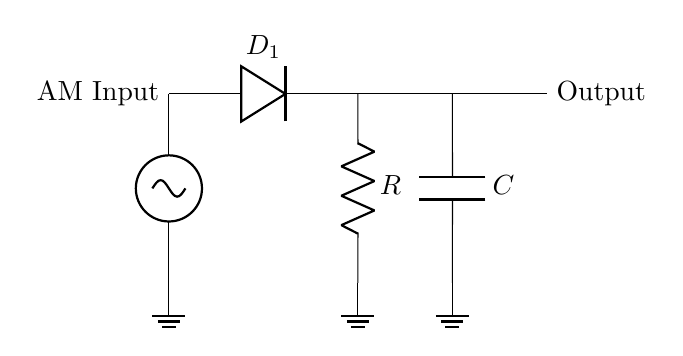
\begin{tikzpicture}[scale=1.2]
        % Circuit
        \draw (0,0) node[left] {AM Input} to[diode, l=$D_1$] (2,0) -- (4,0) node[right] {Output};
        \draw (2,0) to[R, l=$R$] (2,-2) -- (2,-2) node[ground]{};
        \draw (3,0) to[C, l=$C$] (3,-2) -- (3,-2) node[ground]{};
        \draw (0,-2) node[ground]{};
        \draw (0,0) to[sV] (0,-2);
    \end{tikzpicture}
    \end{center}

    \textbf{Working Principle:}

    \begin{center}
    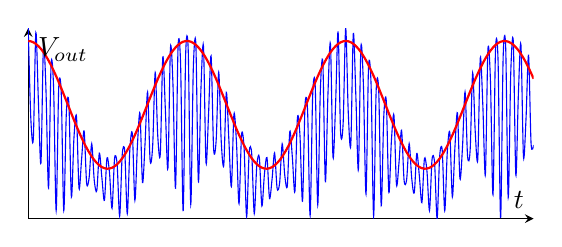
\begin{tikzpicture}
        \begin{axis}[
            width=8cm, height=4cm,
            axis lines=middle,
            xtick=\empty, ytick=\empty,
            xlabel=$t$, ylabel=$V_{out}$,
            domain=0:20, samples=200
        ]
            \addplot[blue, smooth] {(1 + 0.5*cos(deg(x))) * abs(cos(deg(10*x)))};
            \addplot[red, thick, smooth] {1 + 0.5*cos(deg(x)) - 0.1}; % Approximate envelope
        \end{axis}
    \end{tikzpicture}
    \end{center}

    \textbf{Operation:}

    \begin{itemize}
        \item \textbf{Diode Conduction}: Conducts during positive half cycles.
        \item \textbf{Capacitor Charging}: Charges to peak value.
        \item \textbf{RC Discharge}: Discharges through RC circuit.
        \item \textbf{Envelope Following}: Output follows envelope.
    \end{itemize}

    \textbf{Design Considerations:}

    \begin{itemize}
        \item \textbf{Time Constant}: $RC \gg 1/f_c$ but $RC \ll 1/f_m$.
        \item \textbf{Diode Selection}: Fast recovery diode preferred.
        \item \textbf{Load Resistance}: Should be much larger than diode resistance.
    \end{itemize}

    \textbf{Advantages:}

    \begin{itemize}
        \item \textbf{Simplicity}: Very simple circuit.
        \item \textbf{Low Cost}: Economical solution.
        \item \textbf{High Efficiency}: Good detection efficiency.
    \end{itemize}

    \begin{mnemonicbox}
    "Diode Charges, RC Follows Envelope - DCRF"
    \end{mnemonicbox}
\end{solutionbox}

\questionmarks{4}{a}{3}
\textbf{Illustrate under sampling, over sampling and critical sampling.}

\begin{solutionbox}
    \textbf{Answer}:

    \begin{center}
    \begin{tabulary}{\linewidth}{L L L}
        \toprule
        \textbf{Type} & \textbf{Condition} & \textbf{Result} \\
        \midrule
        \textbf{Under Sampling} & $f_s < 2f_m$ & Aliasing occurs \\
        \textbf{Critical Sampling} & $f_s = 2f_m$ & Just adequate, no margin \\
        \textbf{Over Sampling} & $f_s > 2f_m$ & No aliasing, safe margin \\
        \bottomrule
    \end{tabulary}
    \end{center}

    \textbf{Diagram:}

    \begin{center}
    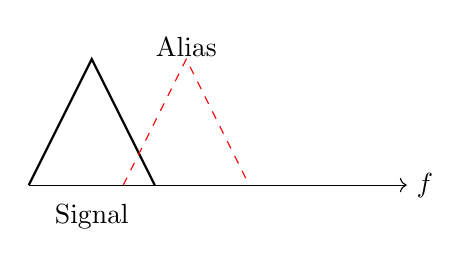
\begin{tikzpicture}[scale=0.8]
        \draw[->] (0,0) -- (6,0) node[right] {$f$};
        \draw[thick] (0,0) -- (1,2) -- (2,0);
        \node at (1,-0.5) {Signal};
        
        % Aliased
        \draw[dashed, red] (1.5,0) -- (2.5,2) -- (3.5,0);
        \node at (2.5, 2.2) {Alias};
    \end{tikzpicture}
    \end{center}

    \begin{itemize}
        \item \textbf{Aliasing Effect}: Under sampling causes frequency overlap.
        \item \textbf{Nyquist Rate}: Minimum sampling rate = $2f_m$.
    \end{itemize}

    \begin{mnemonicbox}
    "Under-Alias, Critical-Just, Over-Safe - UCO"
    \end{mnemonicbox}
\end{solutionbox}

\questionmarks{4}{b}{4}
\textbf{State Sampling theorem and define Nyquist rate, Nyquist interval and aliasing error.}

\begin{solutionbox}
    \textbf{Answer}:

    \textbf{Sampling Theorem:}
    "A continuous signal can be completely recovered from its samples if sampling frequency is at least twice the highest frequency component of the signal."

    \textbf{Definitions:}

    \begin{center}
    \begin{tabulary}{\linewidth}{L L L}
        \toprule
        \textbf{Term} & \textbf{Definition} & \textbf{Formula} \\
        \midrule
        \textbf{Nyquist Rate} & Minimum sampling frequency & $f_s = 2f_m$ \\
        \textbf{Nyquist Interval} & Maximum sampling interval & $T_s = 1/(2f_m)$ \\
        \textbf{Aliasing Error} & Frequency overlap due to under sampling & $f_a = |f_s - f|$ \\
        \bottomrule
    \end{tabulary}
    \end{center}

    \textbf{Mathematical Expression:}

    \begin{itemize}
        \item \textbf{Sampling Frequency}: $f_s \ge 2f_m$ (Nyquist criterion).
        \item \textbf{Sampling Period}: $T_s = 1/f_s$.
        \item \textbf{Aliasing Condition}: $f_s < 2f_m$.
    \end{itemize}

    \begin{mnemonicbox}
    "Sample at twice message frequency - S2M"
    \end{mnemonicbox}
\end{solutionbox}

\questionmarks{4}{c}{7}
\textbf{Discuss Ideal, Natural and Flat top sampling.}

\begin{solutionbox}
    \textbf{Answer}:

    \textbf{Types of Sampling:}

    \begin{center}
    \begin{tabulary}{\linewidth}{L L L}
        \toprule
        \textbf{Type} & \textbf{Characteristics} & \textbf{Mathematical Expression} \\
        \midrule
        \textbf{Ideal Sampling} & Impulse train multiplication & $x_s(t) = x(t) \cdot \delta_T(t)$ \\
        \textbf{Natural Sampling} & Variable width pulses & Top follows signal \\
        \textbf{Flat Top Sampling} & Constant amplitude pulses & Sample and hold \\
        \bottomrule
    \end{tabulary}
    \end{center}

    \textbf{Waveforms:}

    \begin{center}
    \begin{tikzpicture}[scale=0.8]
        % Ideal
        \node[left] at (0,6) {Ideal};
        \foreach \x in {0,1,2,3,4,5,6}
            \draw[->, thick] (\x,5) -- (\x, {5 + 0.5*sin(\x*60)});
            
        % Natural
        \node[left] at (0,3) {Natural};
        \foreach \x in {0,1,2,3,4,5,6}
            \draw[fill=gray!20] (\x-0.1, 2) -- (\x-0.1, {2 + 0.5*sin((\x-0.1)*60)}) -- (\x+0.1, {2 + 0.5*sin((\x+0.1)*60)}) -- (\x+0.1, 2) -- cycle;

        % Flat Top
        \node[left] at (0,0) {Flat Top};
        \foreach \x in {0,1,2,3,4,5,6}
            \draw[fill=gray!20] (\x-0.1, -1) rectangle (\x+0.1, {-1 + 0.5*sin(\x*60)});
    \end{tikzpicture}
    \end{center}

    \textbf{Frequency Spectrum:}
    \begin{itemize}
        \item \textbf{Ideal}: Exact spectral replication.
        \item \textbf{Natural}: Slight spectral modification.
        \item \textbf{Flat Top}: Aperture effect ($Sa(\pi f T/2)$) present.
    \end{itemize}

    \begin{mnemonicbox}
    "Ideal-Impulse, Natural-Variable, Flat-Constant - IVF"
    \end{mnemonicbox}
\end{solutionbox}

\orquestions

\questionmarks{4}{a}{3}
\textbf{Illustrate the working of Delta modulator with suitable block diagram.}

\begin{solutionbox}
    \textbf{Answer}:

    \textbf{Delta Modulator Block Diagram:}

    \begin{center}
    \begin{tikzpicture}[auto, node distance=2cm,>=latex']
        \node [gtu block] (comp) {Comparator};
        \node [gtu block, right of=comp, node distance=3cm] (quant) {1-bit Quantizer};
        \node [coordinate, right of=quant, node distance=2cm] (out) {};
        \node [gtu block, below of=quant] (int) {Integrator};
        \node [gtu block, left of=int, node distance=3cm] (delay) {Delay};
        \node [left of=comp, node distance=2cm] (in) {Input};

        \draw [->] (in) -- (comp);
        \draw [->] (comp) -- (quant);
        \draw [->] (quant) -- (out) node[right] {Output};
        \draw [->] (quant) -- (int);
        \draw [->] (int) -- (delay);
        \draw [->] (delay) -| (comp);
    \end{tikzpicture}
    \end{center}

    \textbf{Working Principle:}

    \begin{itemize}
        \item \textbf{Comparison}: Input compared with previous integrated output.
        \item \textbf{1-bit Quantization}: Output is $+\Delta$ or $-\Delta$.
        \item \textbf{Integration}: Integrator approximates input signal.
    \end{itemize}

    \begin{mnemonicbox}
    "Compare, Quantize, Integrate, Feedback - CQIF"
    \end{mnemonicbox}
\end{solutionbox}

\questionmarks{4}{b}{4}
\textbf{Write disadvantages of Delta modulation (DM) with suitable explanation.}

\begin{solutionbox}
    \textbf{Answer}:

    \begin{center}
    \begin{tabulary}{\linewidth}{L L L}
        \toprule
        \textbf{Disadvantage} & \textbf{Explanation} & \textbf{Solution} \\
        \midrule
        \textbf{Slope Overload} & Cannot track fast changes & Increase step size \\
        \textbf{Granular Noise} & Quantization noise in flat regions & Decrease step size \\
        \textbf{High Bit Rate} & Requires high sampling rate & Use ADPCM \\
        \bottomrule
    \end{tabulary}
    \end{center}

    \textbf{Slope Overload Condition:} When $|dx/dt| > \Delta f_s$.

    \textbf{Waveforms:}

    \begin{center}
    \begin{tikzpicture}[scale=0.8]
        \draw[->] (0,0) -- (6,0) node[right] {$t$};
        \draw[blue, thick] (0,0) sin (1.5, 2) cos (3,0);
        \draw[red, steps] (0,0) -- (0.2,0.2) -- (0.4,0.4) -- (0.6, 0.6) -- (0.8, 0.8) -- (1.0, 1.0);
        \node at (2, 2.2) {Slope Overload};
    \end{tikzpicture}
    \end{center}

    \begin{mnemonicbox}
    "Slope-Overload, Granular-Noise, High-Bitrate - SOG-H"
    \end{mnemonicbox}
\end{solutionbox}

\questionmarks{4}{c}{7}
\textbf{Describe functions of each block of pulse code modulation (PCM) transmitter and receiver.}

\begin{solutionbox}
    \textbf{Answer}:

    \textbf{PCM Transmitter:}

    \begin{center}
    \begin{tikzpicture}[gtu tree]
    \node [gtu block] {Analog Input}
        child {node [gtu block] {LPF}
            child {node [gtu block] {Sample \& Hold}
                child {node [gtu block] {Quantizer}
                    child {node [gtu block] {Encoder}
                        child {node [gtu block] {Digital Output}}
                    }
                }
            }
        };
    \end{tikzpicture}
    \end{center}

    \textbf{PCM Receiver:}

    \begin{center}
    \begin{tikzpicture}[gtu tree]
    \node [gtu block] {Digital Input}
        child {node [gtu block] {Decoder}
            child {node [gtu block] {DAC}
                child {node [gtu block] {LPF}
                    child {node [gtu block] {Analog Output}}
                }
            }
        };
    \end{tikzpicture}
    \end{center}

    \textbf{Block Functions:}

    \begin{itemize}
        \item \textbf{LPF}: Anti-aliasing filter.
        \item \textbf{Sample \& Hold}: Samples signal.
        \item \textbf{Quantizer}: Converts to discrete levels.
        \item \textbf{Encoder}: Converts to binary.
        \item \textbf{Decoder}: Converts binary to levels.
        \item \textbf{DAC}: Digital to Analog.
    \end{itemize}

    \begin{mnemonicbox}
    "LSQE for TX; DCF for RX"
    \end{mnemonicbox}
\end{solutionbox}

\questionmarks{5}{a}{3}
\textbf{Discuss block diagram of TDM-PCM system in brief.}

\begin{solutionbox}
    \textbf{Answer}:

    \textbf{TDM-PCM System Block Diagram:}

    \begin{center}
    \begin{tikzpicture}[gtu tree]
    \node [gtu block] {Channels 1-3}
        child {node [gtu block] {Commutator}
            child {node [gtu block] {PCM Encoder}
                child {node [gtu block] {Transmission}
                    child {node [gtu block] {PCM Decoder}
                        child {node [gtu block] {Decommutator}
                             child {node [gtu block] {Channels 1-3 Output}}
                        }
                    }
                }
            }
        };
    \end{tikzpicture}
    \end{center}

    \textbf{System Operation:}

    \begin{itemize}
        \item \textbf{Commutator}: Sequential sampling.
        \item \textbf{PCM Encoder}: Digitizes samples.
        \item \textbf{Time Division}: Channels get fixed time slots.
        \item \textbf{Decommutator}: Separates channels.
    \end{itemize}

    \begin{mnemonicbox}
    "Time Division Multiple Access - TDMA"
    \end{mnemonicbox}
\end{solutionbox}

\questionmarks{5}{b}{4}
\textbf{Write short note on Adaptive delta modulation (ADM).}

\begin{solutionbox}
    \textbf{Answer}:

    \textbf{ADM Block Diagram:}

    \begin{center}
    \begin{tikzpicture}[auto, node distance=2cm,>=latex']
        \node [gtu block] (comp) {Comparator};
        \node [gtu block, right of=comp, node distance=3cm] (logic) {Logic};
        \node [gtu block, below of=logic] (step) {Step Ctl};
        \node [gtu block, left of=step, node distance=3cm] (int) {Integrator};
        \node [left of=comp] (in) {Input};
        \node [right of=logic] (out) {Output};

        \draw[->] (in) -- (comp);
        \draw[->] (comp) -- (logic);
        \draw[->] (logic) -- (step);
        \draw[->] (step) -- (int);
        \draw[->] (int) -| (comp);
        \draw[->] (logic) -- (out);
    \end{tikzpicture}
    \end{center}

    \textbf{Working Principle:}
    
    \begin{itemize}
        \item \textbf{Adaptive Step Size}: Changes based on slope.
        \item \textbf{Slope Overload}: Increases step size.
        \item \textbf{Granular Noise}: Decreases step size.
    \end{itemize}

    \begin{mnemonicbox}
    "Adaptive Step size Reduces both Slope-overload and Granular noise - ASRSG"
    \end{mnemonicbox}
\end{solutionbox}

\questionmarks{5}{c}{7}
\textbf{Define Line coding. Draw NRZ (unipolar), RZ (unipolar), Manchester coding waveforms for "1 0 1 1 1 0 1 1".}

\begin{solutionbox}
    \textbf{Answer}:

    \textbf{Definition:} Line coding is the process of converting digital data into digital signals suitable for transmission.

    \textbf{Waveform Diagrams (Data: 1 0 1 1 1 0 1 1):}

    \begin{center}
    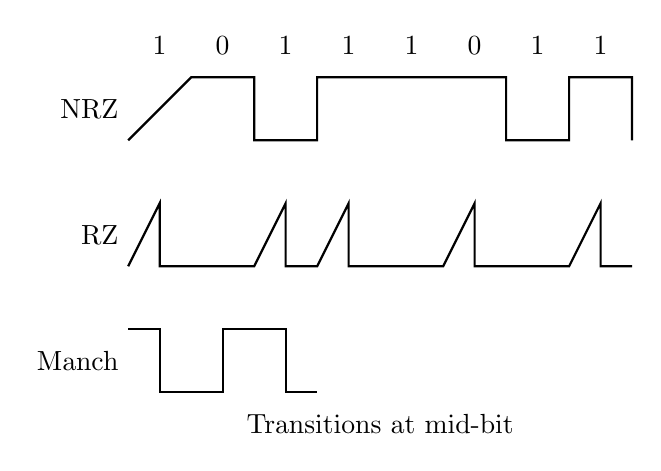
\begin{tikzpicture}[x=0.8cm, y=0.8cm]
        % Data labels
        \foreach \b [count=\i] in {1,0,1,1,1,0,1,1} \node at (\i-0.5, 4.5) {\b};
        
        % NRZ Unipolar
        \node[left] at (0,3.5) {NRZ};
        \draw[thick] (0,3) -- (1,4) -- (2,4) -- (2,3) -- (3,3) -- (3,4) -- (6,4) -- (6,3) -- (7,3) -- (7,4) -- (8,4) -- (8,3);
        
        % RZ Unipolar
        \node[left] at (0,1.5) {RZ};
        \draw[thick] (0,1) -- (0.5,2) -- (0.5,1) -- (1,1) -- (2,1) -- (2.5,2) -- (2.5,1) -- (3,1) -- (3.5,2) -- (3.5,1) -- (5,1) -- (5.5,2) -- (5.5,1) -- (6,1) -- (7,1) -- (7.5,2) -- (7.5,1) -- (8,1);

        % Manchester
        \node[left] at (0,-0.5) {Manch};
        \draw[thick] (0,0) -- (0.5,0) -- (0.5,-1) -- (1,-1) -- (1.5,-1) -- (1.5,0) -- (2,0) -- (2.5,0) -- (2.5,-1) -- (3,-1);
        \node at (4,-1.5) {Transitions at mid-bit};
    \end{tikzpicture}
    \end{center}

    \textbf{Comparison:}

    \begin{center}
    \begin{tabulary}{\linewidth}{L L L}
        \toprule
        \textbf{Type} & \textbf{Logic 1} & \textbf{Logic 0} \\
        \midrule
        \textbf{NRZ} & +V & 0V \\
        \textbf{RZ} & +V for T/2 & 0V \\
        \textbf{Manchester} & High-to-Low & Low-to-High \\
        \bottomrule
    \end{tabulary}
    \end{center}

    \begin{mnemonicbox}
    "NRZ-Simple, RZ-Return, Manchester-Transition - SRT"
    \end{mnemonicbox}
\end{solutionbox}

\orquestions

\questionmarks{5}{a}{3}
\textbf{Describe concept of Time division digital multiplexing.}

\begin{solutionbox}
    \textbf{Answer}:

    \textbf{TDM Concept:} Multiple signals transmitted by allocating different time slots.

    \textbf{Frame Structure:}

    \begin{center}
    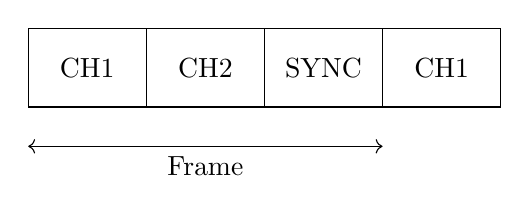
\begin{tikzpicture}
        \draw (0,0) rectangle (1.5,1) node[midway] {CH1};
        \draw (1.5,0) rectangle (3,1) node[midway] {CH2};
        \draw (3,0) rectangle (4.5,1) node[midway] {SYNC};
        \draw (4.5,0) rectangle (6,1) node[midway] {CH1};
        \draw[<->] (0,-0.5) -- (4.5,-0.5) node[midway, below] {Frame};
    \end{tikzpicture}
    \end{center}

    \begin{mnemonicbox}
    "Time slots Share Single Channel - TSSC"
    \end{mnemonicbox}
\end{solutionbox}

\questionmarks{5}{b}{4}
\textbf{Write short note on Differential PCM (DPCM).}

\begin{solutionbox}
    \textbf{Answer}:

    \textbf{DPCM Block Diagram:}

    \begin{center}
    \begin{tikzpicture}[auto, node distance=2cm]
        \node [gtu block] (diff) {Difference};
        \node [gtu block, right of=diff, node distance=3cm] (quant) {Quantizer};
        \node [gtu block, right of=quant, node distance=3cm] (enc) {Encoder};
        \node [gtu block, below of=quant] (dec) {Loc Dec};
        \node [gtu block, left of=dec, node distance=3cm] (pred) {Pred};
        \node [left of=diff] (in) {Input};

        \draw[->] (in) -- (diff);
        \draw[->] (diff) -- (quant);
        \draw[->] (quant) -- (enc);
        \draw[->] (quant) -- (dec);
        \draw[->] (dec) -- (pred);
        \draw[->] (pred) -| (diff);
    \end{tikzpicture}
    \end{center}

    \textbf{Idea:} Use prediction to transmit only difference signal, reducing bit rate.

    \begin{mnemonicbox}
    "Predict Difference, Quantize Less - PDQL"
    \end{mnemonicbox}
\end{solutionbox}

\questionmarks{5}{c}{7}
\textbf{Write short note on 4 level digital multiplexing Hierarchy.}

\begin{solutionbox}
    \textbf{Answer}:

    \textbf{Level Structure:}

    \begin{center}
    \begin{tabulary}{\linewidth}{L L L L}
        \toprule
        \textbf{Level} & \textbf{Bit Rate} & \textbf{Voice Ch} & \textbf{Name} \\
        \midrule
        \textbf{Level 0} & 64 kbps & 1 & DS-0 \\
        \textbf{Level 1} & 1.544 Mbps & 24 & T1 \\
        \textbf{Level 2} & 6.312 Mbps & 96 & T2 \\
        \textbf{Level 3} & 44.736 Mbps & 672 & T3 \\
        \bottomrule
    \end{tabulary}
    \end{center}

    \textbf{Multiplexing Structure:}

    \begin{center}
    \begin{tikzpicture}[gtu tree]
    \node [gtu block] {DS-4}
        child {node [gtu block] {6 x DS-3}
            child {node [gtu block] {7 x DS-2}
                child {node [gtu block] {4 x DS-1}
                    child {node [gtu block] {24 x DS-0}}
                }
            }
        };
    \end{tikzpicture}
    \end{center}

    \begin{mnemonicbox}
    "0-1-2-3 levels Build Communication Systems - DS-BCS"
    \end{mnemonicbox}
\end{solutionbox}

\end{document}
